\section{Our Model}
We use the SLAPP platform for agent simulation,
SLAPP3 provides agent based protocoll in Python 3; specifically: 1observer tempo del mondo - Classi agenti e sui breed(classi derivate) - Usiamo superAgent ch disegna i grafici e crea gli agenti. - azioni generiche gia implementate da specificare a seconda della modellizzazione :DO1.. Draw net... 
\\
\begin{figure}[htpb]
  \centering
  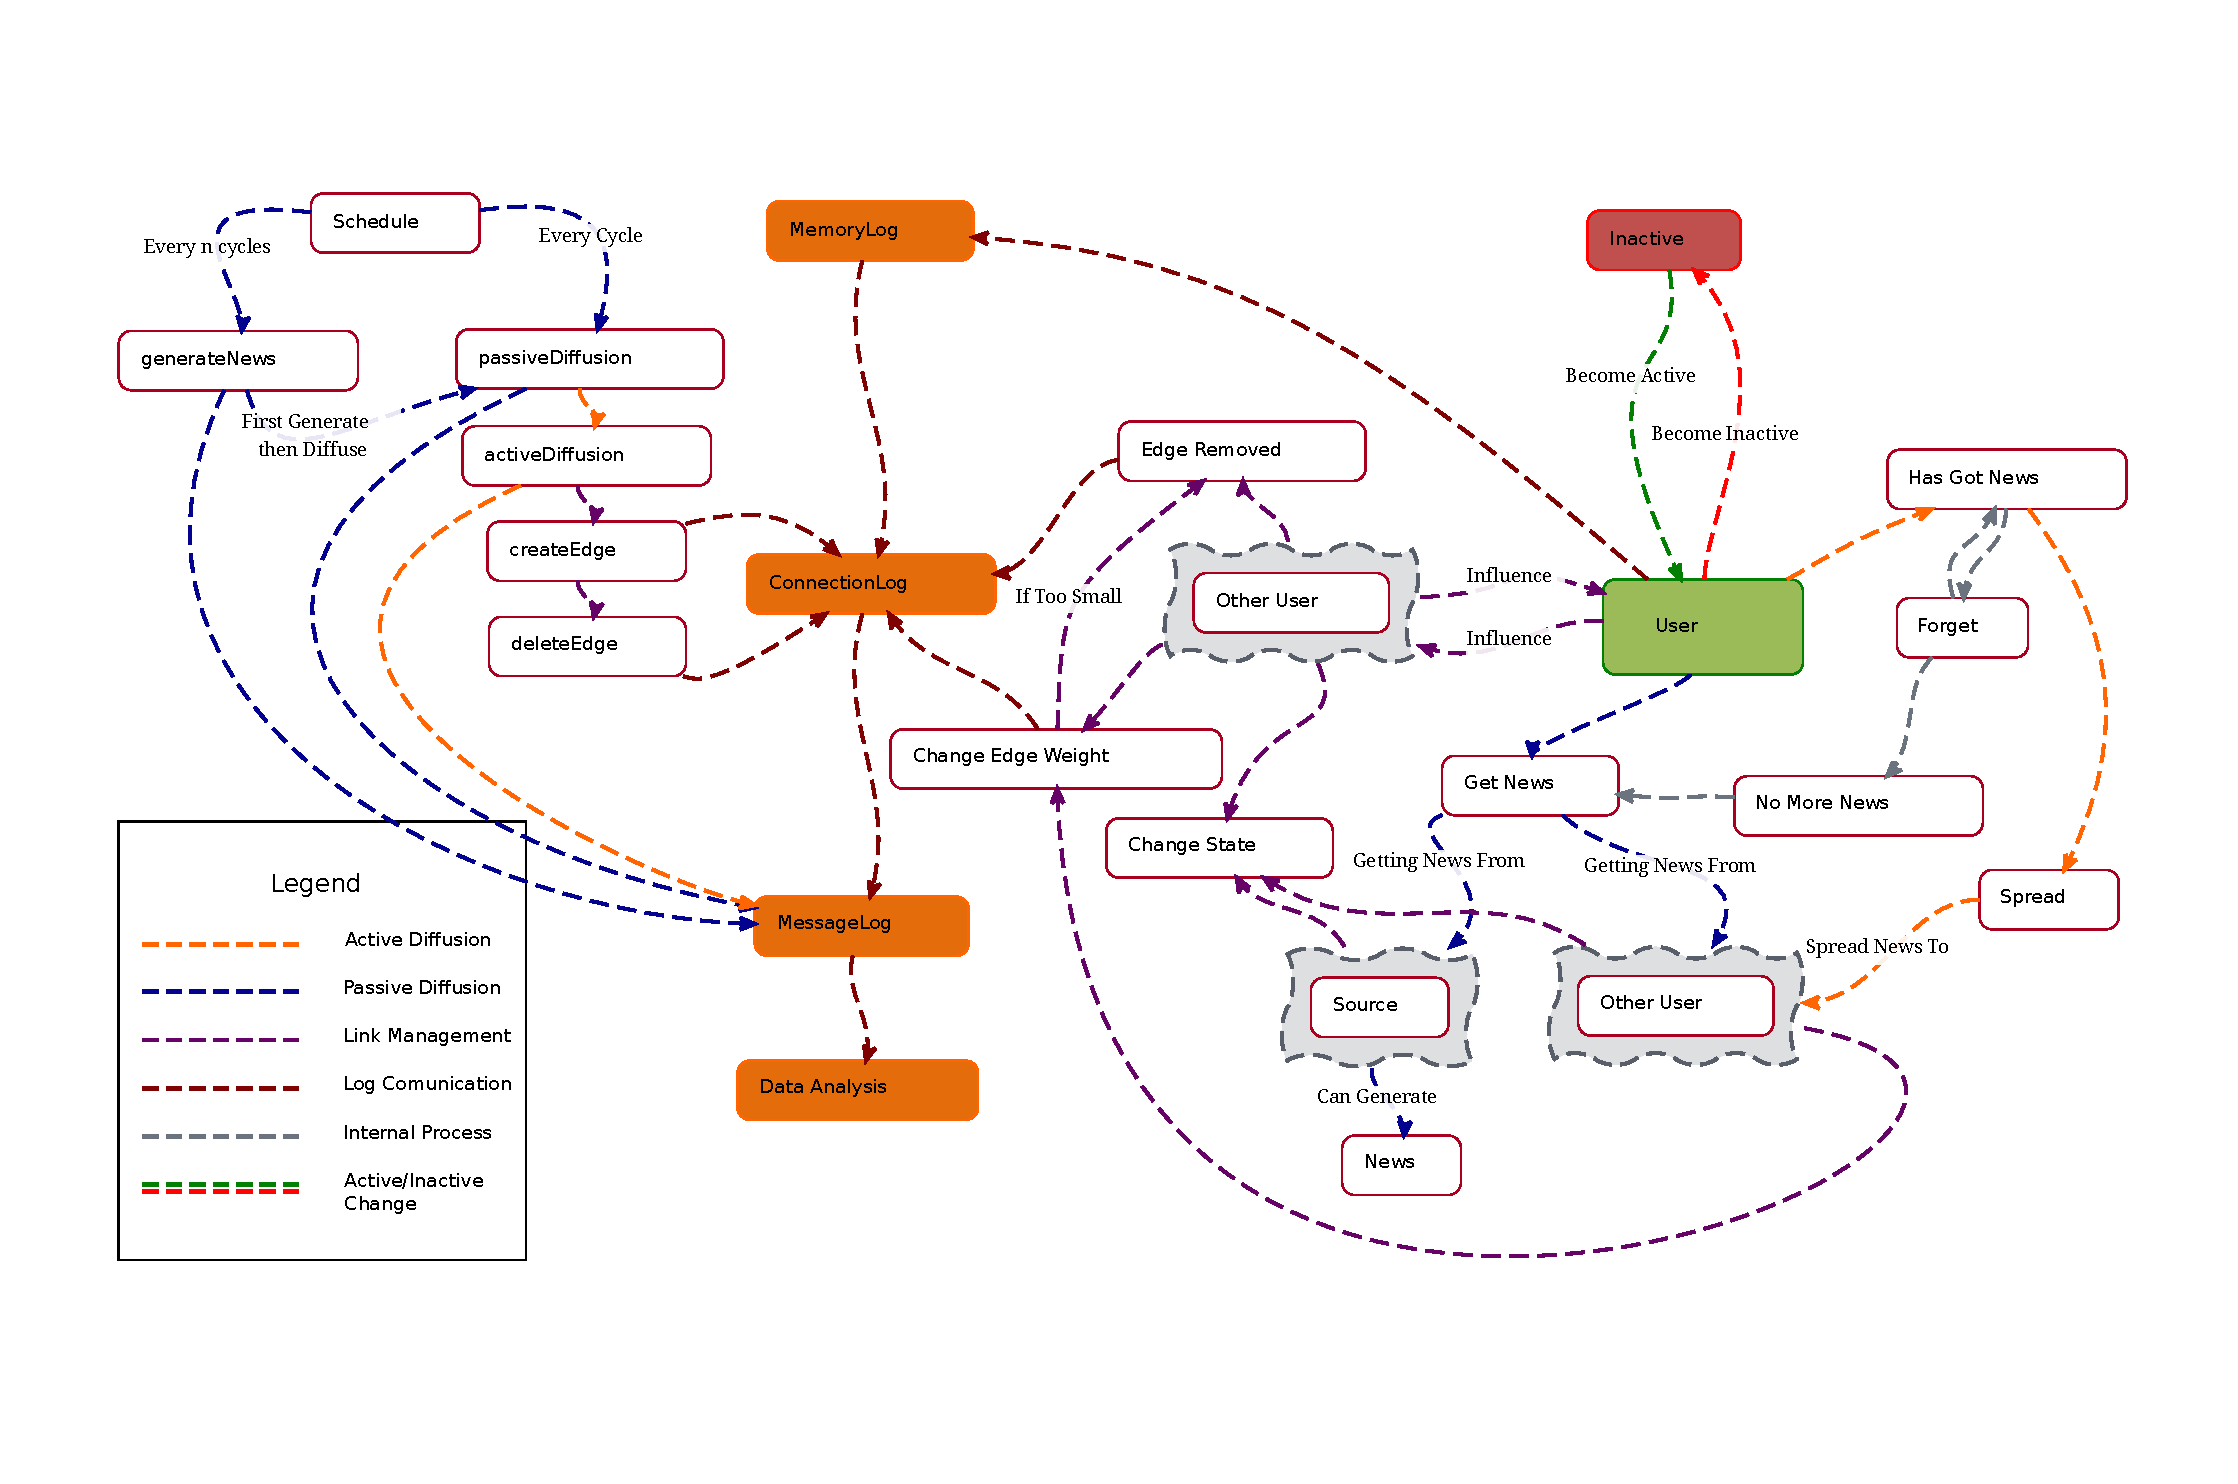
\includegraphics[width=\columnwidth]{mindMap.pdf}
  \label{fig:mindmap}
  \caption{Mind map of the model}
\end{figure}

\begin{tikzpicture}
  \genealogytree[template=signpost]{
    child{
      g{Agent}
      child{
        g{World Agent}
        child{
          g{Users}
        }
        c{Sources}
      }
      %c[phantom=5em]{aaaaaaa}
      child{
        g{Sky Agent}
        child{
          g{Agent Manager}
          child{
            g{Agent Manager\\Message Scheduler\\AMMS}
          }
          c{Agent Manager\\Connection Scheduler\\AMCS}
          c{Agent Manager\\Memory Scheduler\\AMME}
        }
      }
      
    }
  }
\end{tikzpicture}
The agents involved are structured in a hierarchy. 
Schedule: modo per programmare le varie azioni, in ordine temporale esplicitamente dato d noi.  Le azioni possono essere performate con una certa probabilità... removelinks...
Si interfaccia alle azioni generich sopramenzionate.
\\
Le varie Funzioni base (1.2.3.4.5....  9che concatenate costituiscono le azioni vere e proprie degli agenti: Funzioni e metodi delle classi::: SPECCHIETTO
User/Sources
La dinamica del sistema sarà determinata dalle azioni degli utenti; i parametri sopra descritti
influenzeranno le loro decisioni.
\begin{itemize}
\item Agent.py   (user/source) 
\item SkyAgent  (Message scheduler and ConnectionManager ) write the log files...
\item Graph (Create the Graph/ edges and display the graph)
\item Souces
\item Users

\item msglog
\end{itemize}
Funzioni:
Una apposita funzione “distanza” permette di confrontare una notizia con lo stato mentale del
singolo utente; in esso è contenuto un vettore avente come dimensione il numero di topics. Lo stato
contiene inoltre altri parametri che caratterizzano con maggiore specificità il singolo utente, ad
esempio la sua propensione a leggere e diffondere notizie.
